\documentclass[reprint,english,notitlepage]{revtex4-2}  % defines the basic parameters of the document

% if you want a single-column, remove reprint

% allows special characters (including æøå)
\usepackage[utf8]{inputenc}
\usepackage[english]{babel}
\usepackage{float}
%% note that you may need to download some of these packages manually, it depends on your setup.
%% I recommend downloading TeXMaker, because it includes a large library of the most common packages.

\usepackage{physics,amssymb}  % mathematical symbols (physics imports amsmath)
\usepackage{graphicx}         % include graphics such as plots
\usepackage{xcolor}           % set colors
\usepackage{hyperref}         % automagic cross-referencing (this is GODLIKE)
\usepackage{tikz}             % draw figures manually
\usepackage{listings}         % display code
\usepackage{subfigure}        % imports a lot of cool and useful figure commands

% defines the color of hyperref objects
% Blending two colors:  blue!80!black  =  80% blue and 20% black
\hypersetup{ % this is just my personal choice, feel free to change things
    colorlinks,
    linkcolor={red!50!black},
    citecolor={blue!50!black},
    urlcolor={blue!80!black}}

%% Defines the style of the programming listing
%% This is actually my personal template, go ahead and change stuff if you want
\lstset{ %
	inputpath=,
	backgroundcolor=\color{white!88!black},
	basicstyle={\ttfamily\scriptsize},
	commentstyle=\color{magenta},
	language=Python,
	morekeywords={True,False},
	tabsize=4,
	stringstyle=\color{green!55!black},
	frame=single,
	keywordstyle=\color{blue},
	showstringspaces=false,
	columns=fullflexible,
	keepspaces=true}


%% USEFUL LINKS:
%%
%%   UiO LaTeX guides:        https://www.mn.uio.no/ifi/tjenester/it/hjelp/latex/ 
%%   mathematics:             https://en.wikibooks.org/wiki/LaTeX/Mathematics

%%   PHYSICS !                https://mirror.hmc.edu/ctan/macros/latex/contrib/physics/physics.pdf

%%   the basics of Tikz:       https://en.wikibooks.org/wiki/LaTeX/PGF/TikZ
%%   all the colors!:          https://en.wikibooks.org/wiki/LaTeX/Colors
%%   how to draw tables:       https://en.wikibooks.org/wiki/LaTeX/Tables
%%   code listing styles:      https://en.wikibooks.org/wiki/LaTeX/Source_Code_Listings
%%   \includegraphics          https://en.wikibooks.org/wiki/LaTeX/Importing_Graphics
%%   learn more about figures  https://en.wikibooks.org/wiki/LaTeX/Floats,_Figures_and_Captions
%%   automagic bibliography:   https://en.wikibooks.org/wiki/LaTeX/Bibliography_Management  (this one is kinda difficult the first time)
%%   REVTeX Guide:             http://www.physics.csbsju.edu/370/papers/Journal_Style_Manuals/auguide4-1.pdf
%%
%%   (this document is of class "revtex4-1", the REVTeX Guide explains how the class works)


%% CREATING THE .pdf FILE USING LINUX IN THE TERMINAL
%% 
%% [terminal]$ pdflatex template.tex
%%
%% Run the command twice, always.
%% If you want to use \footnote, you need to run these commands (IN THIS SPECIFIC ORDER)
%% 
%% [terminal]$ pdflatex template.tex
%% [terminal]$ bibtex template
%% [terminal]$ pdflatex template.tex
%% [terminal]$ pdflatex template.tex
%%
%% Don't ask me why, I don't know.

\begin{document}
\title{Kvantetilstand i et dobbelt-spalte system}   % self-explanatory
\author{Carl Petter Duedahl}               % self-explanatory
\author{Henrik Modahl Breitenstein}        % self-explanatory
\date{\today}                             % self-explanatory
\noaffiliation                            % ignore this
\begin{abstract}                          % marks the beginning of the abstract
Vi har sett på hvordan en kvantetilstand vil oppføre seg i en boks med en, to og tre spalter ved å gjøre numeriske beregninger. Avviket til den totale sannsynligheten fikk vi til å være på størrelsesordenen $10^{-14}$. Ved to spalter ser vi hvordan kvantetilstanden tidsutvikler seg, ved at noe reflekteres og noe går igjennom splatene. For en, to og tre splater ser vi på sannsynlighetstettheten ved $x=0.8$ og finner at sannsynlighetstetteheten ligner mye på fordelingen til interferenslinjene til bølger igjennom splater.              % the body of the abstract
\end{abstract}                            % marks the end of the abstract
\maketitle                                % creates the title, author, date & abstract

If you want to learn more about using \LaTeX, you should check UiO's official tutorials:
\url{https://www.mn.uio.no/ifi/tjenester/it/hjelp/latex/}

If you are familiar with \LaTeX\ and you want to learn more about the REVTeX4-1 document class, check:
\url{http://www.physics.csbsju.edu/370/papers/Journal_Style_Manuals/auguide4-1.pdf}


% the fundamental components of scientific reports:
\section{Introdukson}
Et viktig eksperiment gjennom historien har vært to-spalte eksperimentet, først introdusert av Thomas Young på 1800-tallet (Referanse 1). Young sitt eksperiment gikk ut på hvordan lys oppfører seg som en bølge. Senere har det blitt vist hvordan partikler, som for eksempel elektroner også kan oppføre seg som bølger ved hjelp av to-spalte eksperimentet. Forståelsen på hvordan en partikkel interferer med seg selv er gitt av Schrödingerlikningen fra kvantefysikken:

\begin{equation}
	i \hbar \frac{d}{dt} |\Psi\rangle = \hat{H} |\Psi\rangle,
\end{equation}

For å kunne se hvordan en kvantetilstand vil oppføre seg i et slikt eksperiment så skal vi bruke Schrödingers likning til å simulere et ett-spalte, to-spalte og tre-spalte system innad i en boks. Ved å gjøre dette kan vi finne sannsylighetsfordelingen til en tenkt partikkel og sammenlikne med tidligere teoretiske og eksperimentelle resultater. I teori delen går igjennom Schrödingerlikningen og Crank-Nicolson likningen. I metode delen viser vi hvordan vi setter opp systemet og ser på hvordan vi tidsutvikler det. Vi representer resultatene så i resultatskapittelet og diskuterer de separat i diskusjonsdelen. Til slutt summerer vi opp og kommer med en konklusjon.
\section{Teori}   % (optional)

\subsection{Om Schrödinger-likningen}
Vi har altså at Schrödinger-likningen kan skrives som
$$
i\hbar\frac{d}{dt}\ket{\Psi}=\hat{H}\ket{\Psi}
$$
Vi skal imidlertid se på en partikkel i et todimensjonalt system med en vegg med et høyt tidsuavhenig potensial $V(x,y)$. Da blir Schrödinger-likningen heller slik
$$
i\hbar \frac{d}{dt}\Psi(x,y,t)=-\frac{\hbar^2}{2m}(\frac{\delta^2}{\delta x^2}+\frac{\delta^2}{\delta y^2})+V(x,y)\Psi(x,y,t)
$$
I denne oppgaven vil vi være mest opptatt av hvordan sannsynligheten for å finne partikkelen på spesifike posisjoner i systemet utvikler seg over tid. Av Borns regel har vi at sansyligheten for å finne partikkelen i en tilstand eller i vårt tilfelle posisjon på et gitt tidspunkt er
$$
p(x,y;t)=|\Psi(x,y,t)|^2=\Psi^*(x,y,t)\Psi(x,y,t)
$$
I denne simuleringen skal vi forenkle denne modellen slik at vi nå har
$$
i\frac{d u}{dt}=-\frac{\delta u}{\delta x}-\frac{\delta u}{\delta y}+v(x,y)u
$$
Her er $u$ en normalisert og dimensjonsløs kvantetilstand. Siden den er normalisert og vi går over et gitter vil da
$$
\sum p_{i,j}=\sum u_{i,j}^*u_{i,j}=1
$$
I tillegg er $u$ i et dimensjonsløst plan så vi setter $x$ og $y$ til å gå fra $0$ til $1$. Selve likningens tilstand vil bli videre diskutert i \autoref{ssec:Init}. $v(x,y)$ er også innenfor det samme enhetsløse to-dimensjonale planet og vil bli videre diskutert i \autoref{ssec:Spalte}.
\subsection{Initialtilstand}
\label{ssec:Init}
Vi trenger en initialtilstand, altså tilstanden $u(x,y,t=0)=u^0_{i,j}$. Vi skal bruke en Gaussisk initialtilstand på formen
$$
u(x,y,t=0)=\frac{1}{C}e^{-\frac{(x-x_c)^2}{2\sigma_x^2}-\frac{(y-y_c)^2}{2\sigma_y^2}+ip_x(x-x_c)+ip_y(y-y_c)}
$$
Siden dette er Gaussisk så vil $x_c$ og $y_c$ være toppunktet til $p_{i,j}$ og der det vil være mest sannsynlig at partikkelen er. $p_x$ og $p_y$ er bevegelsesmengden til partikkelen. $\sigma_x$ og $\sigma_y$ er bredden til funksjonen. $C$ er normaliseringskonstanten. Siden vi skal gjøre dette over et gitter får vi heller
$$
u_{i,j}^0=\frac{1}{C}e^{-\frac{(x_i-x_c)^2}{2\sigma_x^2}-\frac{(y_j-y_c)^2}{2\sigma_y^2}+ip_x(x_i-x_c)+ip_y(y_j-y_c)}
$$
Vi må også normalisere dette, altså at $\sum_{i,j} u^n_{i,j}*u^n_{i,j}=\sum_{i,j}p^n_{i,j}=1$, og så det vi da må gjøre er å la
$$
C=\sum_{i,j}|e^{-\frac{(x_i-x_c)^2}{2\sigma_x^2}-\frac{(y_j-y_c)^2}{2\sigma_y^2}+ip_x(x_i-x_c)+ip_y(y_j-y_c)}|^2
$$
Å normalisere slikt gjør vi kun i initialtilstanden, men dersom systemet er nøyaktig nok, vil $\sum_{i,j}p$ holde seg ganske nærme 1. Imens vi tidsutvikler koden vår vil vi summere opp alle $p_{i,j}$ for å se om den totale sansynligheten holder seg jevnt rundt $1$ og dermed også kontrollere at vi gjør riktig.
\newline Vår matrise vil være på størrelsen $M\cross M$ og dimensjonene vil være normalisert så laveste verdiene av $x $ og $y$ vil være $0$ og høyeste $1$. Vi vil fortsatt bruke Dirichlet grensebetingelser så vi setter $u(x=0,y, t)=u(x=1,y, t)=u(x, y=0, t)=u(x,y=1, t)=0$ uansett tidssteg. Det gjør at vi egentlig ikke trenger å finne tidsutviklingen i grensene så for når begrenser vi $U$ til å være en $(M-2)\cross (M-2)$-matrise, med $u_{0,0}^n=u(x=0+h,y=0+h, t)$ og $u_{M-3,M-3}=u(x=1-h,y=1-h)$. Hvor $h$ da er steglengden.
\subsection{Lage spalten} \label{ssec:Spalte}
Så trenger vi å lage en vegg og en spalteåpning. Vi skal sette spalten i midten av systemet vårt, altså har den et midtpunkt i $x=0,5$. Så skal tykkelsen på veggen være $0,02$ i x-retning. I y-retning har vi da hullene og veggene. Vi vil i starten bruke to spalte, men vil også variere mellom å bruke én spalte, tre spalte og ikke ha noen vegg i det hele tatt. Vi tar først eksempelet med to åpninger. Da har vi først en vegg, så en åpning på $0,05$, deretter et en vegg også på $0,05$, så en ny åpning på $0,05$ og til slutt en vegg som er like lang som den første veggen. Lengden på åpningene og veggene mellom åpningene vil ikke forandre seg når vi endrer antall åpninger, men veggene på sidene vil endre seg avhengig av antall åpninger vi har. For å finne lengden for endeveggene kan vi da bruke
$$
l_{endevegg}=\frac{1-(n_{slits}+n_{mellomvegger})\cdot 0.05}{2}
$$
Vi får da at
\begin{table}[H]
	\begin{tabular}{|c|c|}
		\hline
		Antall åpninger & Endevegg \\
		\hline 
		1 & $0,475$ \\
		\hline
		2& $0,425$ \\ \hline 
		3& $0,375$ \\ \hline
		
	\end{tabular}
\end{table}
Vi går da fra 0 opp til den tilhørende vegglengden og finner høyden åpningen starter i, så går vi $0,05$ opp for å finne hvor skilleveggen starter, så går vi enda $0,05$ opp for å finne hvor neste åpning starter og fortsetter slik for å få til vi når endeveggen. Vi finner da y-verdiene vi trenger og får vegger som i \autoref{fig:Wall1}, \autoref{fig:Wall2} og \autoref{fig:Wall3}.

\begin{figure}[H]
	\centering 
	\includegraphics[scale=0.1]{../Images/1Walls.pdf}
	\caption{Veggenes og åpningenes start og ender på y-aksen i tillegg til veggenes tykkelse. Veggen har her én åpning.}
	\label{fig:Wall1}
\end{figure}
\begin{figure}[H]
	\centering 
	\includegraphics[scale=0.1]{../Images/NewWalls.pdf}
	\caption{Veggenes og åpningenes start og ender på y-aksen i tillegg til veggenes tykkelse. Veggen har her to åpninger}
	\label{fig:Wall2}
\end{figure}

\begin{figure}[H]
	\centering 
	\includegraphics[scale=0.1]{../Images/NewWalls.pdf}
	\caption{Veggenes og åpningenes start og ender på y-aksen i tillegg til veggenes tykkelse. Veggen har her tre åpninger}
	\label{fig:Wall3}
\end{figure}
Vi kan fortsatt ikke generelt anta at slike posisjoner ligger nøyaktig på et punkt på posisjonsgitteret vårt, så vi vil avrunde til det nærmeste punktet. 
\newline Idéelt sett burde veggen hatt et uendelig stort potensial for at veggdelen skulle vært helt ugjennomtrengelig. Dessverre er uendelig et altfor stort tall for maskinen å regne med. Vi setter derfor potensialet der veggen er til å være $10^{10}$, og over resten av systemet vil potensialet være $0$.
\subsection{Numerisk tillnærming} 
V har da fra Schrödingerlikningen at
$$
i\frac{\delta u}{\delta t}=-\frac{\delta^2 u}{\delta x^2}-\frac{\delta^2 u}{\delta y^2}+v(x,y)
$$
eller 
$$
\frac{\delta u}{\delta t}=i\frac{\delta^2 u}{\delta x^2}+i\frac{\delta^2 u}{\delta y^2}-iv(x,y)
$$
Vi skal så bruke Crank-Nicolson tilnærming så vi starter med å approksimere den venstre-siden
$$
\frac{d u}{dt}=\frac{u^{n+1}_{i,j}-u^{n}_{i,j}}{\Delta t}
$$
Hvor $n$ er tidstegt vi er i.
Crank-Nicolson baser seg på forover og bakover tilnærminger. For forover har vi at
$$
\frac{u^{n+1}_{i,j}-u^{n}_{i,j}}{\Delta t}=F^{n}_{i,j}
$$ 
mens bakover har vi
$$
\frac{u^{n+1}_{i,j}-u^{n}_{i,j}}{\Delta t}=F^{n+1}_{i,j}
$$
Så kombinerer vi disse forover og bakover
$$
\frac{u^{n+1}_{i,j}-u^n_{i,j}}{\Delta t}=\theta F^{n+1}_{i,j}-(1-\theta)F^{n}_{i,j}
$$
slik at for $\theta=1$ har vi bakovertilnærmingen og for $\theta=0$ har vi forovertilnærmingen.
For Crank-Nicolson setter vi $\theta =\frac{1}{2}$ slik at vi får
$$
\frac{u^{n+1}_{i,j}-u^n_{i,j}}{\Delta t}=\frac{1}{2}(F^{n+1}_{i,j}-F^{n}_{i,j})
$$

\subsection{Bruke Crank-Nicolson}
Vi hadde fra Crank-Nicolson at
$$
\frac{u^{n+1}_{i,j}-u^n_{i,j}}{\Delta t}=\frac{1}{2}(F^{n+1}_{i,j}-F^{n}_{i,j})
$$
I vårt tilfelle er 
$$
F_{i,j}=i\frac{\delta^2 u}{\delta x^2}+i\frac{\delta^2 u}{\delta y^2}-iv(x,y)u
$$
så 
$$
F^{n}_{i,j}=i\frac{\delta^2 u^n}{\delta x^2}+i\frac{\delta^2 u^n}{\delta y^2}-iv(x,y)u^n
$$
Vi bruker deretter at
$$
\frac{\delta^2 u^n}{\delta x^2}\approx\frac{u^{n}_{i+1,j}-2u^{n}_{i,j}+u^n_{i-1,j}}{\Delta x^2}
$$
Siden $i$ er den eneste som varierer i med hensyn på x, er det denne vi vil bruke her. Tilsvarende får vi at
$$
\frac{\delta^2 u^n}{\delta y^2}=\approx \frac{u^n_{i,j+1}-2u^n_{i,j}+u^{n}_{i,j-1}}{\Delta y^2}
$$
Så vi får da at
$$
F^n=i\begin{pmatrix}
\frac{u^{n}_{i+1,j}-2u^{n}_{i,j}+u^n_{i-1,j}}{\Delta x^2} \\ +\frac{u^n_{i,j+1}-2u^n_{i,j}+u^{n}_{i,j-1}}{\Delta y^2}-v_{i,j}u_{i,j}
\end{pmatrix}
$$
Vi går igjen tilbake til
$$
\frac{u^{n+1}_{i,j}-u^n_{i,j}}{\Delta t}=\frac{1}{2}(F^{n+1}_{i,j}-F^{n}_{i,j})
$$
og flytter over slik at vi får
$$
u^{n+1}_{i,j}-\frac{\Delta t}{2}F^{n+1}_{i,j}=u^{n}_{i,j}+\frac{\Delta t}{2}F^{n}_{i,j}
$$
Vi utvider $F$ og får
$$
\begin{matrix}
	u_{i,j}^{n+1} \\ -\frac{i\Delta t}{2\Delta x^2}(u^{n+1}_{i+1,j}-2u^{n+1}_{i,j}+u^{n+1}_{i-1,j}) \\ -\frac{i\Delta t}{2\Delta y^2}(u^{n+1}_{i,j+1}-2u^{n+1}_{i,j}+u^{n+1}_{i,j-1}) \\ \frac{i\Delta t}{2}v_{i,j}u^{n+1}_{i,j}
\end{matrix}=\begin{matrix}
u^n_{i,j}\\ +\frac{i\Delta t}{2\Delta x^2}(u^{n}_{i+1,j}-2u^{n}_{i,j}+u^{n}_{i-1,j}) \\ +\frac{i\Delta t}{2\Delta y^2}(u^n_{i,j+1}-2u^n_{i,j}+u^{n}_{i,j-1}) \\ -\frac{i\Delta t}{2}v_{i,j}u^n_{i,j} 
\end{matrix}
$$
Vi skal gå over samme steglengde på x og y aksen så vi setter $\Delta x=\Delta y=h$. Så definerer vi $r\equiv \frac{i\Delta t}{2h^2}$ slik at vi har
$$
\begin{matrix}
	u_{i,j}^{n+1} \\ -\frac{i\Delta t}{2\Delta x^2}(u^{n+1}_{i+1,j}-2u^{n+1}_{i,j}+u^{n+1}_{i-1,j}) \\ -r(u^{n+1}_{i,j+1}-2u^{n+1}_{i,j}+u^{n+1}_{i,j-1}) \\ \frac{i\Delta t}{2}v_{i,j}u^{n+1}_{i,j}
\end{matrix}=\begin{matrix}
	u^n_{i,j}\\ +r(u^{n}_{i+1,j}-2u^{n}_{i,j}+u^{n}_{i-1,j}) \\ +r(u^n_{i,j+1}-2u^n_{i,j}+u^{n}_{i,j-1}) \\ -\frac{i\Delta t}{2}v_{i,j}u^n_{i,j} 
\end{matrix}
$$
\subsection{Matriseform}
FOr å gjøre det litt raskere skal vi konvertere om til matriseform som i Kilde 1. Denne gangen har vi imedlertid to dimensjoner så det blir litt annerledes. Første forskjellen er at vi har en todimensjonal matrise med elementer $u_{i,j}$ hvor radene er y-aksen og kollonnene y-aksen, mens vi trenger en vektor for å tidsuvikle ved hjelp av matriser. Vi vil derfor lage en vektor $\vec{u}$ som organiserer matrisen slik
$$
\vec{u}=(u_{0,0}, u_{1,0}, u_{2,0} (...) u_{M-2, 0} u_{0,1},(...) u_{0, M-2}, (...) u_{M-2, M-2})
$$
Så $k=i+j\cdot (M-2)$. Det betyr at $\vec{u}$ er $(M-2)^2$ stor.
\newline 
Vi skal så lage matrisene $A$ og $B$ slik at
$$
B\vec{u}^n=\vec{c}
$$
og
$$
A\vec{c}=\vec{u}^{n+1}
$$
La oss ta et eksempel i $(M-2)=3$. Da vil matrisen $A$ og $B$ være
$$
A=\begin{pmatrix}
	a_0 & -r & 0 & -r & 0 &0&0&0&0 \\
	-r & a_1 & -r & 0 & -r& 0&0&0&0 \\
	0 &-r &a_2&0&0&-r&0&0&0 \\
	-r &0&0&a_3&-r&0&-r&0&0 \\
	0&-r&0&-r&a_4&&-r&0&-r&0 \\
	0&0&-r&0&-r&a_5&0&0&-r \\
	0&0&0&-r&0&0&a_6&-r&0 \\
	0&0&0&0&-r&0&-r&a_7&-r \\
	0&0&0&0&0&-r&0&-r&a_8
\end{pmatrix}
$$
og
$$
B=\begin{pmatrix}
	b_0 & r & 0 & r & 0 &0&0&0&0 \\
	r & b_1 & r & 0 & r& 0&0&0&0 \\
	0 &r &b_2&0&0&r&0&0&0 \\
	r &0&0&b_3&r&0&r&0&0 \\
	0&r&0&r&b_4&&r&0&r&0 \\
	0&0&r&0&r&b_5&0&0&r \\
	0&0&0&r&0&0&b_6&r&0 \\
	0&0&0&0&r&0&r&b_7&r \\
	0&0&0&0&0&r&0&r&b_8
\end{pmatrix}
$$
Hvor diagonalene er satt sammen av vektorene $\vec{a}$ og $\vec{b}$ hvor elementene er gitt som
$$
a_k=1+4r+\frac{i\Delta t}{2}v_{i,j}
$$
og
$$
b_k=1-4r-\frac{i\Delta t}{2}v_{i,j}
$$
Av disse matrisene kan vi se to ting. Foruten om diagonalen er $A=-B$. I tillegg foruten om diagonalene er matrisene satt sammen av to $M-2 \cross M-2$ matriser. Diagonalen til $B$ består av matrisen $P$ med som har side-diagonalene $r$. For $M-2=3$ får vi da at
$$
P=\begin{pmatrix}
	0 &r&0\\
	r &0 &r \\
	0 & r& 0
\end{pmatrix}
$$
Denne matrisen vil gå diagonalt ned over $B$. Som sidediagonaler til denne matrisen, altså under og til venstre for $P$ vil vi har matrisen $R$ som har diagonalen bestående av $r$. Så for $M-2=3$ har vi da
$$
R=\begin{pmatrix}
	r&0&0 \\
	0&r&0 \\
	0&0&r
\end{pmatrix}
$$
Så da har vi uten å ta hensyn til diagonalen at
$$
-A=B=\begin{pmatrix}
	P&R&0 \\
	R&P&0 \\
	0&R&P
\end{pmatrix}
$$
Legger vi så til vektorene $\vec{a}$ og $\vec{b}$ langs diagonalene har vi matrisene $A$ og $B$.
\subsection{Startverdier og tilhørende simuleringer}
Vi har nå laget en funksjon som gir oss en del resultater og er avhengig av en del verdier. En forklaring for alle instillingene finnes i \ref{table:Initverdier}
\begin{table}[H]
	\begin{tabular}{|c|p{20mm}|}
		\hline
		$h$ & Steglengden over x og y-aksen \\\hline 
		$\Delta t$ & Tidsstegene \\\hline 
		$T$ & Den totale tiden vi kjører simuleringen over. \\\hline
		$x_c$ og $y_c$ & Hvor initialtistandens sansynlighet vil være sentrert for deres tilhørende akse. \\\hline 
		$\sigma_x$ og $\sigma_y$ & Bredden til den gaussiske funskjonen intialtilstanden består av. \\\hline 
		$p_x$ og $p_y$ & Bevegelses- mengden i x og y retning for initialtilstanden. \\\hline 
		$v_0$ & Potensialet i veggen. \\\hline
		$n_{slits}$ & Antall åpninger i veggen \\\hline
	\end{tabular}
\caption{En forklaring for alle verdiene som trengs for å kjøre simulasjonen}
\label{table:Initverdier}
\end{table}
I alle tilfeller vi tester vi $h=0,005$ $\Delta t=2,5\cdot 10^{-5}$, $x_c=0,25$, $y_c=0,5$, $\sigma_x=0,05$ og $p_y=0$. De andre vil vi variere.
\subsection{Sansynlighetsunøyaktighet}
Som sagt tidligere burde den totale sansynligheten for å finne partikkelen i systemet holde seg ganske konstant rundt 1. Altså
$$
P^n=\sum_{i,j}p_{i,j}=1
$$
Siden vi dette er numerisk så kan vi få litt avvik fra dette, men jo større dette avviket er, jo verre er modellen vår.  Vi vil derfor som en kontrolltest, sette $v_0=0$ slik at vi ikke har en vegg. Så tester vi med $\sigma_y=0,05$, altså lik som $\sigma_x$. Vi vil da ta $P^n$ for hvert tidssteg og etterpå plotte avviket, altså $P^n-1$. Vi plotter opp til $T=0,008$. Slik har vi en kontrolltest uten noe, så vi ser om sansynligheten holder seg konstant uten en vegg.
\newline Vi legger så til en dobbeltspaltevegg, så $s_l=2$ og $v_0=10^10$. Hvis vi nå fortsetter å ha $\sigma_y=0,05$ vil det meste av bølgefunksjonen gå rett på veggen med samme bredde. Vi setter derfor opp $\sigma_y$ til $0,1$ så en større del av bølgefunksjonen går gjennom spalten. Så kjører vi simulasjonen på nytt og plotter igjen avviket.
\subsection{Simulasjonen i det to dimensjonale tommet}\label{ssec:sim2}
Vi skal så se på $p_{i,j}$ og $u_{i,j}$ i planet. Vi vil her se på noen øyblikksbilder i $t=0$, $t=0,001$ og $t=0,002$. Vi har fortsatt en dobbeltspaltevegg med $v_0=10^10$, men denne gangen har vi $\sigma_y=0,2$.
Vi vil for disse tidstegene plotte den reelle og den imaginære delen av $u_{i,j}$ i planet, og deretter $p_{i,j}=u*_{i,j}u_{i,j}$.
\subsection{Sansynligheten over på en gitt x-verdi}
Vi har også nå de samme startverdiene som fra \autoref{ssec:sim2}. La oss nå anta at ved $t=0,002$ så måler at partikkelen posisjon på x-aksen er $x=0,8$, men vi vet fremdeles ikke partikkelens posisjon på y-aksen. Altså bryter tilstanden sammen til at $p(x=0,5)=1$. Vi vil så finne ut hvordan sansynlighetsfordelingen på y-aksen ved $x=0,5$. Vi bruker forrige simulasjons verdier i $x=0,5$ og normaliserer disse slik at $\sum_{i}u*_iu_i=1$. Så plotter vi over y-aksen. Vi kjører så simulasjonen igjen, $sl=1$ og $sl=3$ og finner sansynlighetsfordelingen over y-aksen i $x=0,8$ for disse også. 
\section{Resultater}
Avviket til den totale sannsyigheten er vist i \autoref{Fig:ToTP} og \autoref{Fig:ToTPs1}

\begin{figure}
	\centering
	\includegraphics[scale=0.4, trim={2cm 0 0 0}]{../Images/7P199.pdf}
	\caption{Avviket til den totale sannsynligheten $1 - P$ for $v_0 = 0 \; m/s$.}
	\label{Fig:ToTP}
\end{figure}

\begin{figure}
	\centering
	\includegraphics[scale=0.4, trim={2cm 0 0 0}]{../Images/7s1P199.pdf}
	\caption{Avviket til den totale sannsynligheten $1 - P$ for $v_0 = 10^10 \; m/s$.}
	\label{Fig:ToTPs1}
\end{figure}

For to-spalte system så fikk vi \autoref{Fig:s2u2t0} for $t = 0 \; s$, med den reelle delen vist i \autoref{Fig:s2u2t0Re} og imaginær i \autoref{Fig:s2u2t0Im}:

\begin{figure}[H]
	\centering
	\includegraphics[scale=0.45, trim={3cm 0 0 0}]{../Images/ImshowUt00sl2.pdf}
	\caption{$|u|^2 $ i tiden $t = 0 \; s$.}
	\label{Fig:s2u2t0}
\end{figure}


\begin{figure}[H]
	\centering
	\includegraphics[scale=0.45, trim={3cm 0 0 0}]{../Images/ImshowRe00sl2.pdf}
	\caption{$Re(u) $ i tiden $t = 0 \; s$.}
	\label{Fig:s2u2t0Re}
\end{figure}


\begin{figure}[H]
	\centering
	\includegraphics[scale=0.45, trim={3cm 0 0 0}]{../Images/ImshowIm00sl2.pdf}
	\caption{$Im(u) $ i tiden $t = 0 \; s$.}
	\label{Fig:s2u2t0Im}
\end{figure}


Ved tiden $t = 0,001 \; s$ fikk vi \autoref{Fig:s2u2t01}:

\begin{figure}[H]
	\centering
	\includegraphics[scale=0.45, trim={3cm 0 0 0}]{../Images/ImshowUt0001sl2.pdf}
	\caption{$|u|^2 $ i tiden $t = 0,001 \; s$.}
	\label{Fig:s2u2t01}
\end{figure}

\begin{figure}[H]
	\centering
	\includegraphics[scale=0.45, trim={3cm 0 0 0}]{../Images/ImshowRe0001sl2.pdf}
	\caption{$Re(u) $ i tiden $t = 0,001 \; s$.}
	\label{Fig:s2Ret01}
\end{figure}

\begin{figure}[H]
	\centering
	\includegraphics[scale=0.45, trim={3cm 0 0 0}]{../Images/ImshowIm0001sl2.pdf}
	\caption{$Im(u) $ i tiden $t = 0,001 \; s$.}
	\label{Fig:s2Imt01}
\end{figure}


Ved tiden $t = 0,002 \; s$ fikk vi \autoref{Fig:s2u2t02} for sannsynlighetsfordelingen og \autoref{s2Ret02} for den relle delen og \autoref{Fig:s2Imt01} for den imaginære:

\begin{figure}[H]
	\centering
	\includegraphics[scale=0.45, trim={3cm 0 0 0}]{../Images/ImshowUt0002sl2.pdf}
	\caption{$|u|^2 $ i tiden $t = 0,002 \; s$.}
	\label{Fig:s2u2t02}
\end{figure}

\begin{figure}[H]
	\centering
	\includegraphics[scale=0.45, trim={3cm 0 0 0}]{../Images/ImshowRe0002sl2.pdf}
	\caption{$Re(u) $ i tiden $t = 0,002 \; s$.}
	\label{Fig:s2Ret02}
\end{figure}

\begin{figure}[H]
	\centering
	\includegraphics[scale=0.45, trim={3cm 0 0 0}]{../Images/ImshowIm0002sl2.pdf}
	\caption{$Im(u) $ i tiden $t = 0,002 \; s$.}
	\label{Fig:s2Imt02}
\end{figure}

Med en spalte så fikk vi sannsynlighetstettheten langs y-aksen for $x = 0.8$ i \autoref{Fig:Ps1}

\begin{figure}[H]
	\centering
	\includegraphics[scale=0.4]{../Images/ScreenProb1Slit.pdf}
	\caption{Sannsnynlighetstettheten ved $x = 0.8$ og $t = 0.001975 \; s$ for en spalte}
	\label{Fig:Ps1}
\end{figure}

For to spalter fikk vi \autoref{Fig:Ps2} og for tre fikk vi \autoref{Fig:Ps3}


\begin{figure}[H]
	\centering
	\includegraphics[scale=0.4]{../Images/ScreenProb2Slit.pdf}
	\caption{Sannsnynlighetstettheten ved $x = 0.8$ og $t = 0.002 \; s$ for to spalter}
	\label{Fig:Ps2}
\end{figure}


\begin{figure}[H]
	\centering
	\includegraphics[scale=0.4]{../Images/ScreenProb3Slit.pdf}
	\caption{Sannsnynlighetstettheten ved $x = 0.8$ og $t = 0.002 \; s$ for tre spalter}
	\label{Fig:Ps3}
\end{figure}

\section{Diskusjon}
\subsection{Sannsynlighetsavvik}
Av \autoref{ToTP} og \autoref{Fig:ToTPs1} ser vi at avviket for den totale sannsynligheten er på en skala av $10^{-14}$ både med og uten vegg, som forsterker troen på at vi har gjort det riktig, siden den totale sansynligheten viker så lite fra 1. $10^{-14}$ begynner også å nærme seg maskinpresisjonen for doubles som vi brukte, altså $10^{-15}$, så det blir vanskelig å få mere nøyaktighet. Vi ser også av \ref{fig:ToTP} at avviket ser ut til å ha en syklus, men kommer seg fortsatt ikke opp mot 0 igjen ved $t=T=0,008$. Dette kan tyde på at avviket blir større, men det kan også hende at avviket blir mindre igjen etter $t=0,008$, men siden vi bare har målt til $t=0,008$ er dette vanskelig å si. I vårt tidsrom er fortsatt avviket lite nok til at man kan si dette er akseptabelt. I \autoref{Fig:ToTPs1} ser det imedlertid ut til at avviket stabiliserer seg ved $t=0,002$. Vi vet igjen ikke hvordan den vil oppføre seg etter $t=0,008$, men for tidsperioden av vår simulering er dette akseptabelt. Så ut ifra sannsynlighetsavviket kan det tyde på at vi har ganske riktige resultater. 
\subsection{Målingene av u i planet}
Av \autoref{Fig:s2u2t0} ser vi en ganske normal todimensjonal sansynlighetsfordeling med et toppunkt i $x_c, y_c$. Ser vi imedlertid på den relle delen og den imaganiære delen for seg som i \autoref{Fig:s2u2t0Re} og \autoref{Fig:s2u2t0Im}, ser vi $|u|^2=p$ egentlig er satt sammen av to bølgefunksjoner som ser ut til å sirkulere på $x$-aksen og har en bredde på $y$-aksen. Ser vi kun på $p$ ser vi at i $t=0,001$ så går noe av $p$ gjennom åpningene, mens noe blir reflektert i veggen og går motsatt vei, som bølger. Til slutt ved $t=0,002$ ser vi i \autoref{Fig:s2u2t02} at $p$ har blitt splittet opp til mindre toppunkter rundt om i planet. De fleste og mest sannsynlige punktene er igjen på venstre side, mens noe har fortsatt gått over til høyre side.
\newline
Ser vi derimot på den reelle og den imaginære delen i \autoref{Fig:s2Ret01} og \autoref{Fig:s2Imt01} ser vi her at det ikke bare er en stråle som $p$ på samme tidspunkt, men at det faktisk her er som bølger som går gjennom en åpning. Når vi også ser på den relle delen og den imaginære delen til $u$ for $t=0,002$ i \autoref{Fig:s2Ret02} og \autoref{Fig:s2Imt02}, så ser vi at det er bølger som har spredd seg, med noen interferenslinjer som er de som synes i \autoref{Fig:s2u2t02}.
\subsection{Sannsynligheten i $x=0,8$}
Vi ser at \autoref{Fig:Ps1} har ett toppunkt, \autoref{Fig:Ps2} har tre og \autoref{Fig:Ps3} har 5. Disse ligner veldig mye på interferenslinjene til bølger som går gjennom spalter som kan forsterke påstanden om at simulasjonen er korrekt, siden vi så at $u$ var satt sammen av bølger. 
\section{Konklusjon}
Vi har simulert oppførelsen til en kvantetilstand i en boks. Ved å gi en initialhastighet så har vi sett hvordan en, to og tre spalter gjør med kvantetilstanden. Avviket til den totale sannsnyligheten i beregningene er på $10^{-14}$. I en boks med dobbeltspalte har vi sett hvordan den imaginære og relle delen av kvantetilstanden er to bølgefunksjoner som kavntetilstanden besttår av. Sannsynlighetstettheten i dobbeltspalte-oppsettet har vi sett splitter seg opp ved at noe går igjennom spaltene imens en annen del blir reflektert av barrieren. For en, to og tre spalter har vi sett nærmere på sannsynlighetstetteheten ved $x = 0.8$, hvor vi får en fordeling som ligner mye på interferensmønsteret for vanlige bølger igjennom spalter.
% acknowledgements (optional)
\begin{acknowledgments}  % if you disagree with the spelling, blame Americans
I would like thank myself for writing this beautiful document.
\end{acknowledgments}


%% When it comes to the bibliography I personally generate it using BibLaTeX. (see the link above if you're interested)
%% You're obviously allowed to create the references section however you like.
%% I'll keep it simple here.
\section*{References}  % the asterisk (*) after \section makes the section numbering go away
\begin{itemize}
\item[-]Reference 1
\item[-]Reference 2
\end{itemize}

\newpage
%% if you want to include an appendix, this is how you do it
\appendix
\section{Name of appendix}
This will be the body of the appendix.
\section{This is another appendix}\label{appendix}
Tada.
%% all \section commands following \appendix are automatically taken as appendices

%% Note that \label{appendix} command on line 115. What this does is setup a reference point for LaTeX that you can
%% access wherever you want using \ref{appendix}.
%% You can place labels on most environments such as equations, figures, tables, etc.

\clearpage
Note that this document is written in the two-column format. If you want to display a large equation, a large figure, or whatever, in one-column format, you can do this like so:
\onecolumngrid
\vspace{1cm} % some extra space
This text and this equation are both in one-column format.

\footnote{This equation is actually from quantum mechanics. ``It's called Schrödinger's Time-Dependent Wave Equation'', named after the awesome Austrian physicist Erwin Rudolf Josef Alexander Schrödinger. Yep, the ``Schrödinger's cat'' guy. Pretty cool dude actually, check his wiki page: \url{https://en.wikipedia.org/wiki/Erwin_Schrodinger}. He was physics' no. 1 Ladies' man if there ever was one. Anyway, you will learn more about this equation in FYS2140. You can also find it printed on a glass wall in the UiO Physics Building (it really is that important).}

\begin{equation}\label{equation}
\frac{-\hbar^2}{2m}\laplacian{\Psi}+V\Psi=i\hbar\pdv{t}\Psi
\end{equation}
Note that the equation numbering (this: \ref{equation}) follows the appendix as this text is technically inside Appendix \ref{appendix}. If you want a detailed listing of (almost) every available math command, check: \url{https://en.wikibooks.org/wiki/LaTeX/Mathematics}.
\vspace{1cm} % some extra space
\twocolumngrid
And now we're back to two-column format. It's really easy to switch between the two. It's recommended to keep the two-column format, because it is easier to read, it's not very cluttered, etc. Pro Tip: You should also get used to working with REVTeX because it is really helpful in FYS2150.

One last thing, this is a code listing:
\begin{lstlisting}
This will be displayed with a cool programming font!
\end{lstlisting}
You can add extra arguments using optional parameters:
\begin{lstlisting}[morekeywords={cool}]
This will be displayed with a cool programming font!
\end{lstlisting}
You can also list code from a file using \texttt{lstinputlisting}. If you're interested, check \url{https://en.wikibooks.org/wiki/LaTeX/Source_Code_Listings}.

This is a basic table:
\begin{table}[h]  % h = "here"  , h! = here!
\caption{This is a nice table}\label{table}
\begin{tabular}{|c|c|c|} % note that & separates columns while \\ separates the rows
\hline                    % creates a horizontal line (try removing it)
Hey & Hey & Hey  \\
\hline
Hello & Hello & Hello \\
\hline
Bye & Bye & Bye \\
\hline
\end{tabular}
\end{table}\\
You can a detailed description of tables here: \url{https://en.wikibooks.org/wiki/LaTeX/Tables}.

I'm not going to delve into Tikz in any level detail, but here's a quick picture:
\begin{figure}[h]
\centering  % places the tikz image in the center of the text column
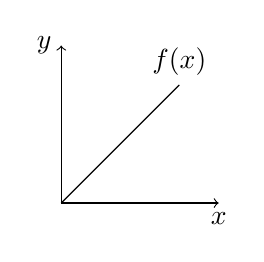
\begin{tikzpicture}
\draw[->] (0,0) -- (2,0) node [pos=1.0,below] {\(x\)};
\draw[->] (0,0) -- (0,2) node [pos=1.0,left] {\(y\)};
\draw (0,0) -- (1.5,1.5) node [pos=1.0,above] {\(f(x)\)};
\end{tikzpicture}
\caption{This is great caption}\label{figure}
\end{figure}\\
If you want to know more, check: \url{https://en.wikibooks.org/wiki/LaTeX/PGF/TikZ}.

%% If you want to include figure:
%\includegraphics[scale=1.0]{filename}
%% check https://en.wikibooks.org/wiki/LaTeX/Importing_Graphics if you want to know more

\end{document}
